\documentclass[11pt,a4paper]{article}
\usepackage[margin=26mm]{geometry}
\usepackage{amsmath,amssymb,amsthm,booktabs,graphicx}
\usepackage{xcolor}
\usepackage[colorlinks=true,linkcolor=blue!45!black,citecolor=blue!45!black,urlcolor=blue!45!black]{hyperref}
\usepackage{microtype}
\newtheorem{proposition}{Proposition}
\newtheorem{theorem}{Theorem}
\newcommand{\E}{\mathbb{E}}
\newcommand{\dd}{\mathrm{d}}
\setlength{\emergencystretch}{2em}
\title{A noise-scaling window for concentration of a shared flow}
\author{David Galbraith}
\date{Revised draft, 11 September 2026}
\begin{document}
\maketitle
\begin{abstract}
Uniform microscopic activity need not give every flow channel equal disturbance:
channels coupled to more interactions can collect more fluctuations. We connect this mechanism
to a conditional prediction for concentrated sharing of a fixed total flow.
For reflected driftless dynamics with flow weight $g^m$ and variance rate
proportional to $g^q/\sum_jg_j^m$, we derive the exact joint stationary law.
The population fraction above the pooled half-flow threshold vanishes as both
state range and population grow precisely when $1\le q\le m+1$, for exact powers.
At fixed population $N$, it instead approaches $1/(2N)$ inside that window.
Independent interaction contributions proportional to actual flow recover $q=m$;
existing deterministic lattice examples demonstrate seeding and flow-dependent
variation, without establishing the complete diffusion limit or both boundaries.
The window concerns scaling across channel states, not overall noise amplitude.
We state finite-range physical tests, including an amplitude-rescaling null.
The power-law moment threshold is established mathematics; the contribution is
its exact conserved-flow formulation and testable physical interpretation.
Physical applicability remains untested.
\end{abstract}

\section{The physical prediction}

Can the same microscopic activity, acting throughout a substrate, sort a fixed
flow into a small fraction of large-share channels? A route coupled to more
microscopic interactions can collect more perturbations under the same local rule. This paper asks
when that state-dependent disturbance permits extreme concentration. It addresses
sharing among available routes; it does not derive the formation of those routes.

The proposed prediction is conditional: physical systems with the flow and
fluctuation laws specified below should follow the finite-range concentration
curve, with asymptotic separation only in the scaling window $1\le q\le m+1$.
This is more specific than the statement that disturbance helps channels grow.
Outside the window, a vanishing population fraction does not carry half the pooled
flow as the accessible range grows. Unequal sharing can nevertheless remain.

The distinction between scaling and amount is essential. After accounting for
the shared normalization, doubling channel state multiplies flow weight by $2^m$
and variance rate by $2^q$. The exponent $q$ concerns variance, not the size of a
typical kick, which scales with its square root. Increasing activity equally at
every interaction multiplies all variance rates by a constant. In this model that
speeds up evolution without changing the stationary distribution. It cannot by
itself traverse the window. The physical question is how coupling to microscopic activity and its
correlations make disturbance increase across channel states.

Noise-dependent residence times and stationary occupation have a long history
\cite{landauer,maes}. Power-weighting a power-law distribution gives a standard
moment threshold; Newman discusses both this condition and the fraction of a
weighted total held by a population tail \cite{newman}. These ingredients are
not claimed as new. Shared-flow normalization also changes the dynamical clock.
Making it explicit gives the exact joint law, finite-population correction and
observable needed to assess this physical mechanism.

\section{A model with conservation imposed at every instant}

Let $N\geq1$ channels have dimensionless states $g_i\in[1,R]$, where $R>1$.
The model specifies possible flow routes and their response law; it does not
prescribe which routes become dominant. The deterministic example in Sec.~\ref{sec:contact} tests differentiation
from identical coarse-route states.
Spatial formation and connectivity of routes in a material are abstracted out:
no spatial energy-gradient field or changing network topology is modeled here.
For $m>0$, define the total weight $S$ and the actual flow through channel $i$ by
\begin{equation}
 S(\mathbf g)=\sum_{j=1}^N g_j^m,\qquad
 J_i(\mathbf g)=I\frac{g_i^m}{S(\mathbf g)}.
 \label{eq:share}
\end{equation}
Thus $\sum_i J_i=I$ for every configuration, not only in expectation. We choose
the interior dynamics
\begin{equation}
 \dd g_i=\sqrt{2D_i(\mathbf g)}\,\dd W_i,\qquad
 D_i(\mathbf g)=\frac{N g_i^q}{S(\mathbf g)},
 \label{eq:model}
\end{equation}
with independent Wiener processes, normal reflection at both endpoints, and
zero interior drift. Boundary local-time terms are implicit. A positive common
prefactor has been absorbed into the time unit. The lower cutoff sets the state
unit; all powers refer to this specified coordinate.

The normalization in Eq.~\eqref{eq:model} is a constitutive assumption. On the
line $q=m$, $D_i=(N/I)J_i$, so noise variance rate is proportional to actual
flow. Away from that line the model keeps the common factor $1/S$. The apparently
similar choice $D_i\propto J_i^{q/m}$ instead contains $S^{-q/m}$ and defines
different dynamics. Conservation of flow alone does not select either rule.

The It\^o convention would follow from an appropriate small-kick limit of
conditionally unbiased additive events in $g$, evaluated at the pre-event
state. Such a limit also needs control of temporal correlations and higher
moments. Unresolved deterministic dynamics do not automatically satisfy these
conditions. Under a nonlinear change $y=h(g)$, It\^o's formula adds the drift
$D(g)h''(g)$ even when the drift in $g$ is zero. The zero-drift assumption must
therefore be justified in the measured coordinate, rather than restored after
arbitrary relabelling.

\section{From uniform microscopic activity to differential disturbance}
\label{sec:contact}

Let each microscopic contribution be conditionally unbiased, with the same
variance $v\,\dd t$ in the specified state coordinate. For $n_i$ independent
contributions, variance addition gives $2D_i=n_iv$. More generally,
\begin{equation}
 \operatorname{Var}\!\left(\sum_{a=1}^{n_i}\xi_a\right)
 =\sum_a\operatorname{Var}(\xi_a)+2\sum_{a<b}\operatorname{Cov}(\xi_a,\xi_b).
 \label{eq:contacts}
\end{equation}
Thus uniform local activity can produce unequal coarse disturbance through
interaction number and correlations. Here $n_i$ is an effective count of coupled
contributions, not a surface area or a spatial dimension. The lattice can index
unresolved degrees of freedom rather than physical positions. A spatial contact
footprint is one realization; the event construction below instead uses interaction
rates. Statistical uniformity means equal microscopic
rules and statistics, not identical states or synchronized trajectories.

If the coupling obeys $n_i=M J_i/I=M g_i^m/S$, independence gives
$D_i=(Mv/2)g_i^m/S$. A common choice of time unit recovers Eq.~\eqref{eq:model}
with $q=m$. Here differential noise follows from the interaction rule rather than
being specified separately for each channel. This line lies in the concentration
window for $m\ge1$; it lies below it for $0<m<1$. More interactions alone are therefore
not a universal sufficient condition.

One explicit small-kick construction gives the same connection. At total rate
$2N/h^2$, an identical interaction event chooses route $i$ with probability $J_i/I$
and adds $+h$ or $-h$ with equal probability; attempted outward moves are rejected.
Each allowed signed jump then has rate $Ng_i^m/(Sh^2)$, the lattice approximation
to the $q=m$ diffusion. Event placement implements the flow-dependent coupling. That coupling is a
constitutive assumption; the variance scaling then follows without specifying
channel geometry. This identifies
the target coarse generator; its event statistics still need to be recovered
from the deterministic substrate.

The repository's deterministic footprint example instead sums fluctuations from
chaotic patches with fixed coupling per patch and footprint proportional to flow
share. It gives a variance-versus-mean-share slope of $1.01$, consistent with
independent variance addition. A separate deterministic example starts forty
coarse routes identically: three fine-state seeds yield final top-three shares
$.615$, $.463$ and $.529$, against $.075$ initially and in frozen controls.
No random numbers are drawn during evolution. The latter example prescribes a
share-dependent amplitude, so it is a seeding demonstration rather than an
independent derivation of contact growth. A periodic control also concentrates;
chaos is not shown necessary.

These examples establish parts of the mechanism, not a complete match to the
bounded diffusion. Their regressions use route-wise time averages; their boundaries
and temporal correlations differ. Deterministic diffusion limits have established
precedents \cite{melbourne,gottwald}, but require conditions not verified here.
Perfectly coherent contributions would give variance proportional to $n_i^2$;
with $n_i\propto J_i$, that also changes the shared denominator to $S^2$.
It cannot be substituted into this theorem by changing $q$ alone. A microscopic
construction crossing both boundaries under the same normalization remains open.

\section{Exact stationary population and flow distributions}

On $[1,R]$, write
\begin{equation}
 Z_R=\int_1^R g^{-q}\dd g,\quad p_0(g)=\frac{g^{-q}}{Z_R},\quad
 \mu_R=\int_1^R g^m p_0(g)\dd g,\quad
 f_R(g)=\frac{g^m p_0(g)}{\mu_R}.
 \label{eq:base}
\end{equation}
All quantities are finite at finite $R$, for every real $q$.

\begin{proposition}
The unique stationary density of Eq.~\eqref{eq:model} on the reflecting box is
\begin{equation}
 \pi_{N,R}(\mathbf g)=\frac{S(\mathbf g)}{N\mu_R}
                 \prod_{j=1}^N p_0(g_j).
 \label{eq:joint}
\end{equation}
Its tagged-channel marginal and its pooled flow density are, respectively,
\begin{align}
 p_{N,R}(g)&=\left(1-\frac1N\right)p_0(g)+\frac1N f_R(g),
 \label{eq:marginal}\\
 \E_{\pi}\!\left[\sum_{i=1}^N\frac{J_i}{I}\delta(g-g_i)\right]&=f_R(g).
 \label{eq:flow}
\end{align}
\end{proposition}

\begin{proof}
Integration of $S\prod_j p_0(g_j)$ gives $N\mu_R$, establishing normalization.
For each coordinate,
\[
 D_i\pi_{N,R}=\frac{1}{Z_R\mu_R}\prod_{j\ne i}p_0(g_j)
\]
is independent of $g_i$. Every probability current
$-\partial_i(D_i\pi_{N,R})$ therefore vanishes, including at the boundaries.
The diffusion is uniformly nondegenerate on the connected compact box, giving
uniqueness. Expanding the sum $S$ and integrating out the other coordinates
gives Eq.~\eqref{eq:marginal}. Multiplication by $J_i/I=g_i^m/S$ cancels $S$
in the joint law; integration and summation give Eq.~\eqref{eq:flow}.
\end{proof}

The calculation also has a simple clock interpretation. If
$L_0=\sum_i g_i^q\partial_i^2$ is the generator of independent reflected
channels, the coupled generator is $L=(N/S)L_0$. Configurations with larger
$S$ are traversed more slowly relative to that independent process; their
stationary weight acquires the factor $S$. This explains both the solvability
and the dependence of the result on the chosen normalization.

An exact independent sampling construction is useful: choose one channel
uniformly, draw its state from $f_R$, and draw the other $N-1$ states independently
from $p_0$. Averaging over the chosen channel reproduces Eq.~\eqref{eq:joint}.
That designation is resampled for each configuration; it does not identify a
permanent winner.

The correction matters even in simple cases. For $N=1$ and $q=m$, the channel
carries all the flow and has constant diffusivity. Its stationary density is
uniform, not $g^{-m}$. At fixed $R$, the tagged marginal approaches $p_0$ as
$N\to\infty$. The independent-channel calculation is recovered in that limit.

\section{The concentration observable and its window}

Let $a_R$ be the state threshold above which half of the pooled flow lies:
\begin{equation}
 \int_{a_R}^R f_R(g)\dd g=\frac12.
\end{equation}
Define $P_0(R)=\int_{a_R}^R p_0(g)\dd g$ and
$P_N(R)=\int_{a_R}^R p_{N,R}(g)\dd g$. Equation~\eqref{eq:marginal} gives
\begin{equation}
 \boxed{P_N(R)=\left(1-\frac1N\right)P_0(R)+\frac{1}{2N}.}
 \label{eq:correction}
\end{equation}
This counts a population fraction above one threshold fixed across stationary
observations. It is a pooled observable, with each observation weighted equally
in physical time.

\begin{theorem}
For Eqs.~\eqref{eq:share}--\eqref{eq:model} with exact powers and $m>0$,
$P_N(R)\to0$ as both $R\to\infty$ and $N\to\infty$ if and only if
\begin{equation}
 \boxed{1\leq q\leq m+1.}
 \label{eq:window}
\end{equation}
At fixed $N$, the limit inside this window is $1/(2N)$.
\end{theorem}

\begin{proof}
Put $A=m-q+1$ and $B=1-q$. Direct integration gives
\begin{equation}
 a_R=\begin{cases}
 [(R^A+1)/2]^{1/A},&A\ne0,\\
 \sqrt R,&A=0,
 \end{cases}\qquad
 P_0(R)=\begin{cases}
 (R^B-a_R^B)/(R^B-1),&B\ne0,\\
 \log(R/a_R)/\log R,&B=0.
 \end{cases}
 \label{eq:quantile}
\end{equation}
For $q<1$, $a_R/R\to2^{-1/A}$ and
$P_0\to1-2^{-B/A}>0$. At $q=1$,
$P_0\sim\log2/(m\log R)\to0$. For $1<q<m+1$, $a_R$ grows proportionally
to $R$, while the normalized population tail above it vanishes.
At $q=m+1$, $P_0=1/(R^{m/2}+1)\to0$.
For $q>m+1$, $a_R\to2^{1/(q-m-1)}$, so
$P_0\to2^{-(q-1)/(q-m-1)}>0$.
Equation~\eqref{eq:correction} supplies the finite-$N$ result and the joint limit.
\end{proof}

Either iterated limit gives this classification, as does any sequence with both
$R$ and $N$ tending to infinity. Stationarity is taken at each bounded pair
$(N,R)$ first. No unbounded diffusion or uniform equilibration time is asserted.
The same classification holds for any fixed pooled flow fraction strictly
between zero and one, with the corresponding fraction divided by $N$ replacing
$1/(2N)$.

The integrals behind the two edges are $\int g^{-q}\dd g$ and
$\int g^{m-q}\dd g$. At the lower edge the population normalization is
logarithmic; at the upper edge the flow normalization is logarithmic.
The upper-edge population fraction itself decays as a power of $R$.
Figure~\ref{fig:window} displays the finite-range expressions.

\begin{figure}[t]
\centering
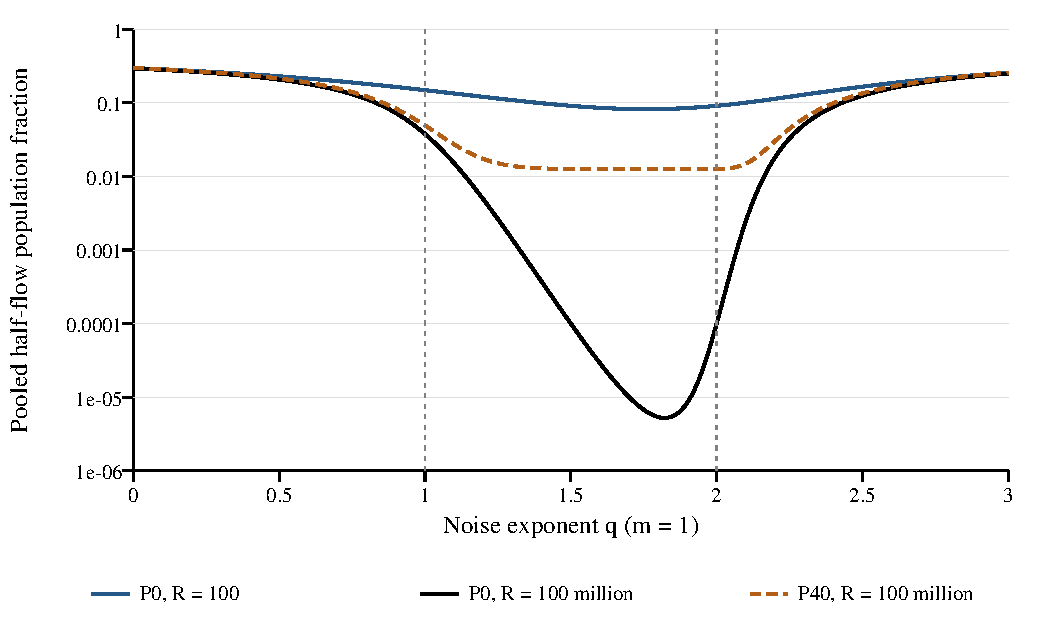
\includegraphics[width=0.94\textwidth]{window_figure.pdf}
\caption{Exact stationary predictions, not empirical measurements or large-range
dynamic simulations. The asymptotic window is between the dotted lines. Finite
range smooths both boundaries; finite population supplies a floor. $P_0$ is the
large-population limit at each fixed $R$. The curve at $R=10^8$ is not the
infinite-range limit.}
\label{fig:window}
\end{figure}

\subsection{Pooled concentration is not a snapshot winner count}

In a single configuration, rank shares in descending order and count the
smallest number of whole channels whose shares sum to at least one half.
Call that count divided by $N$ $H_N$. It always satisfies $H_N\geq1/N$.
In contrast, $P_N$ can approach $1/(2N)$ because its fixed threshold need not
carry half the flow in every snapshot. These observables must not be substituted
for one another. The numerical checks measure $\E H_N$ separately against the
exact joint sampler. Neither statistic measures how long a particular channel
remains dominant. Stationary concentration alone establishes neither persistent
structure nor Darwinian selection.

For example, at $m=1$, $q=2$, $R=10^8$, $P_0\simeq0.000100$, whereas
$P_{40}\simeq0.012598$. This is a substantial relative correction to the tail
fraction, even though $1/N$ is small.

\subsection{Limiting slopes do not determine the endpoints}

The inclusive endpoints require exact powers or additional tail assumptions.
On $g\geq e$, consider the unnormalized flow weight $w(g)=g$ and noise factor
$d(g)=g^2(\log g)^2$. Their limiting log-log slopes are $m=1$ and $q=2$, but
$\int_e^\infty w(g)/d(g)\dd g$ converges. The upper-edge separation fails.
This example also fits the coupled construction with $S=\sum_i w(g_i)$ and
$D_i=N d(g_i)/S$: replace $p_0$ by the normalized $1/d$ and $f_R$ by the
normalized $w/d$ in the proof. Logarithmic corrections do not change the strict
interior power inequalities, but can decide the boundary cases. An estimated
slope near an edge is consequently insufficient to classify a measured system.

\section{What would make the result physically useful?}

The upper bound excludes a proposed mechanism when the measured disturbance
scaling is too steep relative to the flow weight, provided the rest of the model
applies. It also distinguishes state-dependent disturbance from monotonic
reinforcement intuition. At $m=1$, the large-range, large-population half-flow
fraction vanishes for $q=2$, but approaches $1/8$ for $q=2.5$.
Above the boundary it can still be very small, especially close to $q=2$.
The mathematical transition is the loss of a vanishing fraction, not an abrupt
return to equal sharing in a finite apparatus.

The basic inequality is a standard power-law moment condition \cite{newman}.
Its value here is the connection to actual conserved shares and the observable
correction in Eq.~\eqref{eq:correction}. These make a conditional prediction
that can be checked. They do not establish a new general law of nature, and no
priority claim for the elementary threshold is made.

A fair physical test needs simultaneous channel states and individual flows,
with a fixed total and a stable channel population. It must estimate both
conditional drift and variance rate in the chosen coordinate, check cross-channel
correlations, and allow enough relaxation before comparing stationary statistics.
For Eq.~\eqref{eq:model}, conditioning on the configuration or accounting for $S$
is necessary: a regression on $g_i$ alone need not recover $q$. Drift, measurement
noise, jumps, changing populations and limited state range can each prevent the
test from addressing this model. Power-law fits themselves also need checks
against alternatives \cite{clauset}.

The discriminating test has two parts. First, vary a common activity prefactor
at fixed interaction law: after adequate relaxation, the stationary curve should
remain unchanged. Second, vary the state dependence of interaction-driven disturbance,
while verifying the same shared normalization, and compare the finite-range
curve across the upper edge. Fit the dynamical parameters without fitting the
concentration outcome; predict that outcome on separate observations. Change $R$
and, where feasible, $N$ to distinguish a finite-range effect from the asymptotic
classification. No finite apparatus should exhibit an exact singular boundary.

A failed model-assumption check means that this experiment does not test this
particular prediction. Conversely, disagreement with the finite-range curve after
independent checks of those assumptions would count against the proposed model.
No physical dataset is used as validation in this paper.

\section{Numerical checks of the stationary result}

The repository implements a continuous-time nearest-neighbour chain on a uniform
state lattice with spacing $h$. Each allowed jump of channel $i$ by $+h$ or $-h$
has rate
\begin{equation}
 \lambda_i(\mathbf g)=\frac{N g_i^q}{S(\mathbf g)h^2}.
\end{equation}
Outward boundary jumps are absent. Exponential holding times and rate-weighted
event selection simulate this finite chain without a time-step approximation.
The lattice invariant law is exactly Eq.~\eqref{eq:joint} with sums replacing
integrals. Grid refinement remains necessary for a continuous-state comparison.
Observations are taken at fixed physical times, because sampling only jump
events would bias residence-time statistics.

Eight automated tests include detailed balance on every edge of an enumerated
three-channel, three-state system; independent marginal calculations; the
single-channel case; the finite-population quantile identity; sampling checks;
continuum integral comparisons; grid refinement; and relaxation from both
boundaries in a simple control. The retained ensemble runs use six exponent pairs:
$(1,0.5)$, $(1,1)$, $(1,1.5)$, $(1,2)$, $(1,2.5)$ and $(2,4)$.
For each pair they use lower-boundary, upper-boundary, log-uniform and exact
stationary initial conditions, with three seeds and 128 independent ensembles
per seed. Physical observation times are $0,1,4,16$.

\begin{table}[!ht]
\centering
\begin{tabular}{rrrrr}
\toprule
$N$ & Grid intervals & Occupancy CDF & Flow CDF & Mean snapshot fraction\\
\midrule
8 & 4 & 0.017014 & 0.021730 & 0.011423\\
8 & 8 & 0.020299 & 0.024502 & 0.005979\\
40 & 8 & 0.009496 & 0.008539 & 0.001585\\
\bottomrule
\end{tabular}
\caption{Largest final absolute errors across the six exponent pairs and four
initial conditions for each retained run, all on $[1,3]$. CDF errors compare
with the exact lattice law. The snapshot reference uses 100,000 independent
joint-law samples per pair. Seeds are pooled at the final observation time.}
\label{tab:checks}
\end{table}

All retained final errors are below the declared tolerance of $0.05$
(Table~\ref{tab:checks}). This is an acceptance criterion, not a confidence
interval. Separate exact-law calculations check grid refinement and evaluate
large state ranges; they are not dynamical runs at those ranges. The checks
support the implementation on the tested bounded grids. They do not establish
large-range equilibration times or empirical applicability.

The legacy independent-walker check started at the target stationary law
(log-uniform at $q=1$). It did not establish relaxation and is excluded here.

\section{Conclusion}

Uniform microscopic activity can give channels coupled to more interactions
stronger state fluctuations, without reference to a particular spatial geometry. Under the specified conserved-flow dynamics, their
stationary residence times yield an exact concentration window and a measurable
finite-population correction. The upper edge limits extreme pooled concentration;
it does not forbid all large channels or unequal sharing. The proposed physical
test concerns the interaction mechanism, its conditional variance law and the resulting
finite-range curve. It is not a universal amplitude window, a theorem of channel
formation or a derivation of biological selection.

\paragraph{Code and reproducibility.}
Sources, tests, retained data and reproduction commands are at
\url{https://github.com/divadwg/selection-as-physics}; see \texttt{paper/README.md}.

\begin{thebibliography}{99}
\bibitem{landauer} R. Landauer, Motion out of noisy states,
\emph{J. Stat. Phys.} \textbf{53}, 233--248 (1988).
\href{https://doi.org/10.1007/BF01011555}{doi:10.1007/BF01011555}.
\bibitem{maes} C. Maes and K. Neto\v{c}n\'y, Heat bounds and the blowtorch theorem,
\emph{Ann. Henri Poincar\'e} \textbf{14}, 1193--1202 (2013).
\href{https://arxiv.org/abs/1207.1122}{arXiv:1207.1122}.
\bibitem{newman} M. E. J. Newman, Power laws, Pareto distributions and Zipf's law,
\emph{Contemporary Physics} \textbf{46}, 323--351 (2005).
\href{https://arxiv.org/abs/cond-mat/0412004}{arXiv:cond-mat/0412004}.
\bibitem{clauset} A. Clauset, C. R. Shalizi and M. E. J. Newman,
Power-law distributions in empirical data,
\emph{SIAM Review} \textbf{51}, 661--703 (2009).
\href{https://arxiv.org/abs/0706.1062}{arXiv:0706.1062}.
\bibitem{melbourne} I. Melbourne and A. M. Stuart,
A note on diffusion limits of chaotic skew-product flows,
\emph{Nonlinearity} \textbf{24}, 1361--1367 (2011), corrected version (2015).
\href{https://arxiv.org/abs/1101.3087}{arXiv:1101.3087}.
\bibitem{gottwald} G. A. Gottwald and I. Melbourne,
Homogenization for deterministic maps and multiplicative noise,
\emph{Proc. R. Soc. A} \textbf{469}, 20130201 (2013), corrected version (2015).
\href{https://arxiv.org/abs/1304.6222}{arXiv:1304.6222}.
\end{thebibliography}
\end{document}
